%% Vorlage Bachelorarbeit

%% Versionshistorie:

%% v1.0: Erstellung durch Johannes Woske, IT2010
%% v2.0: Überarbeitung und Ergänzung durch Anne Traulsen, IT2015
%% v3.0: Überarbeitung und Anpassung an aktuelles HWR Layout durch Maximilian Bieleke

\documentclass[
	12pt, %Schriftgröße
	a4paper,
	liststotoc, %Inhaltsverzeichniseinträge für Listen (z.B. Abbildungen)
	bibtotoc,%Inhaltsverzeichniseinträge f+r Quellen 
	pointlessnumbers, %Entfernt Punkt hinter Gliederungsnummern
	ngerman, %Sprachpaket
	headsepline, %Headertrennlinie
	%footsepline, %Footertrennlinie
	oneside
    %einseitiges Druckformat %%% Unterdrücken der leeren Seite nach Titelblatt
	]{scrbook} %Dokumentenklasse (Koma-Script)
\author{Marten Tietje}
\usepackage[T1]{fontenc}
\usepackage{float}
\usepackage[utf8]{inputenc}
\usepackage[ngerman]{babel}
\usepackage[
    left = \textquotedblleft{},
    right = \textquotedblright{}, 
    leftsub = \textquoteleft{}, 
    rightsub = \textquoteright{},
]{dirtytalk}

\usepackage{etoolbox}
\makeatletter
\patchcmd{\chapter}{\if@openright\cleardoublepage\else\clearpage\fi}{}{}{}
\makeatother

\usepackage{pdfpages}

\usepackage{lmodern}
\usepackage{markdown}
%Kopf und Fußzeile bearbeiten
\usepackage{fancyhdr}
\pagestyle{fancyplain}
\fancyhf{}
\fancyhead[R]{\thepage}
\renewcommand{\headrulewidth}{0pt}

\usepackage{chronology}
\usepackage{url}
\usepackage{graphicx} %Bilder einfügen
\usepackage{float}
\usepackage{microtype}
%margin für den Header
%\usepackage[a4paper, total={6in, 8in}]{geometry}
\usepackage[a4paper, lmargin=2.1cm, rmargin=3.5cm, tmargin=3cm, bmargin=2cm]{geometry}
%\usepackage[a4paper, margin=1in, headsep=2in]{geometry}
\usepackage[right]{eurosym} %Euro-Zeichen
\usepackage{amssymb}
\usepackage{babel}
\usepackage{fontenc}
\usepackage{graphicx}
\usepackage{csquotes}
\usepackage[
    natbib=true,
    style=apa,
    sorting=none,
    language=ngerman,
    hyperref=true,
]{biblatex}

\defbibenvironment{bibliography}
{\enumerate{}
{\setlength{\leftmargin}{\bibhang}%
\setlength{\itemindent}{-\leftmargin}%
\setlength{\itemsep}{\bibitemsep}%
\setlength{\parsep}{\bibparsep}}}
{\endenumerate}
{\item}

\usepackage[onehalfspacing]{setspace} % Zeilenabstand
\usepackage[ 
   colorlinks,        % Links ohne Umrandungen in zu wählender Farbe 
   linkcolor=black,   % Farbe interner Verweise 
   filecolor=black,   % Farbe externer Verweise 
   citecolor=black,   % Farbe von Zitaten 
   urlcolor=blue	    % Farbe von Links
   ]{hyperref} %Verlinkungen
\usepackage[figure]{hypcap}
\usepackage[toc,page]{appendix}
%\usepackage[titletoc]{appendix}
\usepackage[ngerman]{translator}
\usepackage{listings,xcolor} %Codeanzeige
%\usepackage[nottoc,numbib]{tocbibind}


\lstset{literate=
  {á}{{\'a}}1 {é}{{\'e}}1 {í}{{\'i}}1 {ó}{{\'o}}1 {ú}{{\'u}}1
  {Á}{{\'A}}1 {É}{{\'E}}1 {Í}{{\'I}}1 {Ó}{{\'O}}1 {Ú}{{\'U}}1
  {à}{{\`a}}1 {è}{{\`e}}1 {ì}{{\`i}}1 {ò}{{\`o}}1 {ù}{{\`u}}1
  {À}{{\`A}}1 {È}{{\'E}}1 {Ì}{{\`I}}1 {Ò}{{\`O}}1 {Ù}{{\`U}}1
  {ä}{{\"a}}1 {ë}{{\"e}}1 {ï}{{\"i}}1 {ö}{{\"o}}1 {ü}{{\"u}}1
  {Ä}{{\"A}}1 {Ë}{{\"E}}1 {Ï}{{\"I}}1 {Ö}{{\"O}}1 {Ü}{{\"U}}1
  {â}{{\^a}}1 {ê}{{\^e}}1 {î}{{\^i}}1 {ô}{{\^o}}1 {û}{{\^u}}1
  {Â}{{\^A}}1 {Ê}{{\^E}}1 {Î}{{\^I}}1 {Ô}{{\^O}}1 {Û}{{\^U}}1
  {Ã}{{\~A}}1 {ã}{{\~a}}1 {Õ}{{\~O}}1 {õ}{{\~o}}1
  {œ}{{\oe}}1 {Œ}{{\OE}}1 {æ}{{\ae}}1 {Æ}{{\AE}}1 {ß}{{\ss}}1
  {ű}{{\H{u}}}1 {Ű}{{\H{U}}}1 {ő}{{\H{o}}}1 {Ő}{{\H{O}}}1
  {ç}{{\c c}}1 {Ç}{{\c C}}1 {ø}{{\o}}1 {å}{{\r a}}1 {Å}{{\r A}}1
  {€}{{\euro}}1 {£}{{\pounds}}1 {«}{{\guillemotleft}}1
  {»}{{\guillemotright}}1 {ñ}{{\~n}}1 {Ñ}{{\~N}}1 {¿}{{?`}}1
}

\usepackage{moreverb}
\usepackage{color}




\newcommand\quickwordcount{%
  \immediate\write18{texcount -inc -incbib -sum -1 01_einleitung.tex 02_hauptteil.tex 03_schluss.tex > main-wordcount.sum}\input{main-wordcount.sum}Wörter%
}


\usepackage{chngcntr}
\usepackage{verbatim}
\usepackage{wrapfig}
\counterwithout{figure}{chapter}
\counterwithout{table}{chapter}
\usepackage[acronym]{glossaries}
% \usepackage{mathptmx} % times new roman font schriftart
 

\lstset{ %
  backgroundcolor=\color{white},   % choose the background color
  basicstyle=\footnotesize,        % size of fonts used for the code
  breaklines=true,                 % automatic line breaking only at whitespace
  captionpos=b,                    % sets the caption-position to bottom
  commentstyle=\color{mygreen},    % comment style
  escapeinside={\%*}{*)},          % if you want to add LaTeX within your code
  keywordstyle=\color{blue},       % keyword style
  stringstyle=\color{mymauve},     % string literal style
}
%%%%%%%%%%%%%%%%%%%%%%%%%%%%%%%%%%%%%%%%%%%%%%%%%%%%%
%%%%%%%%%%% Sonderformatierung
%%%%%%%%%%%%%%%%%%%%%%%%%%%%%%%%%%%%%%%%%%%%%%%%%%%%%

% Hurenkinder und Schusterjungen verhindern (Ja, das heißt wirklich so!!)
\clubpenalty = 10000 \widowpenalty = 10000 \displaywidowpenalty = 10000 

\newcommand{\footfigref}[1]{\footnote{Fig. \ref{#1} on page \pageref{#1}}}

%% Bei Referenzen im Text wird jetzt bei allen Ebenen "Kapitel" vorgestellt, z.b. Kapitel 2, Kapitel 2.2, Kapitel 6.3.2
\addto\extrasngerman{%
    \def\sectionautorefname{Kapitel}%
    \def\subsectionautorefname{Kapitel}%
    \def\subsubsectionautorefname{Kapitel}%
    }

% Vertikaler Abstand zwischen Ende Textblock - Ende Fußzeile --> Abstand der Seitenzahl von Rand erhöhen 
\setlength{\footskip}{10mm}

% Abstand vor/nach Überschriften verändern

\RedeclareSectionCommand[%
    beforeskip=0\baselineskip,
    afterskip=0.5\baselineskip
]{chapter}

\RedeclareSectionCommand[%
    beforeskip=0.5\baselineskip,
    afterskip=0.5\baselineskip
]{section}

\RedeclareSectionCommand[%
    beforeskip=0.1\baselineskip,
    afterskip=0.1\baselineskip
]{subsection}

\RedeclareSectionCommand[%
    beforeskip=0.01\baselineskip,
    %%afterskip=0.2\baselineskip
]{paragraph}

\setlength{\abovecaptionskip}{4pt}  % 1pc=12pt 
\setlength{\belowcaptionskip}{0pt}
%\setlength{\textfloatsep}{4pt}
\setlength{\intextsep}{1pc}

%% Verkleinerung der Textgröße unter Abbildungen
\addtokomafont{caption}{\small}

% Den Punkt am Ende der Glossareinträge deaktivieren
\renewcommand*{\glspostdescription}{}

%Glossar-Befehle anschalten

% sorgt dafür, dass bei Leerzeile die Einrückung verhindert und stattdessen eine Leerzeile eingefügt wird % erspart bigskips und erhöht die Lesbarkeit im LaTeX-Text 
\KOMAoptions{parskip=full*}

% ändert Titelschriftart in Serifen-Normalschriftart
\addtokomafont{disposition}{\rmfamily} 
%%%%%%%%%%%%%%%%%%%%%%%%%%%%%%%%%%%%%%%%%%%%%%%%%%%%%
%%%%%%%%%%% Textbausteine
%%%%%%%%%%%%%%%%%%%%%%%%%%%%%%%%%%%%%%%%%%%%%%%%%%%%%
%%%%%%%%%%%% Studentenname
\newcommand{\studentName}{Tietje Marten}
%%%%%%%%%%%% Matr.-Nr.
\newcommand{\matrikelNummer}{686733}
%%%%%%%%%%%% Typ der Arbeit
\newcommand{\type}{Hausarbeit}
%%%%%%%%%%%% Thema
\newcommand{\topic}{Optimierung in der Prozessautomatisierung}
%%%%%%%%%%%% Untertitel
\newcommand{\subtopic}{Integration zwischen SAP Signavio und SAP Build Process Automation am Beispiel von BPMN-Datentransfer}
%%%%%%%%%%%% Studienbereich
\newcommand{\fachbereich}{Duales Studium · Wirtschaft}
%%%%%%%%%%%% Fachrichtung
\newcommand{\fachrichtung}{Wirtschaftsinformatik}
%%%%%%%%%%%% Betrieb
\newcommand{\company}{SAP SE}
%%%%%%%%%%%% Betreuer HWR
\newcommand{\betreuerHS}{Prof. Dr. Claudia Lemke}
%%%%%%%%%%%% Jahrgang
\newcommand{\jahrgang}{2022}
%%%%%%%%%%%% Semester
\newcommand{\semester}{4}
%%%%%%%%%%%% Wordcount
\newcommand{\wordcount}{\quickwordcount}

%init counter
\newcounter{originalpagenumber}

\addbibresource{../assets/literature/sources.bib}


\glstoctrue
%\makenoidxglossaries



%%%%%%%%%%%%%%%%%%%%%%%%%%%%%%%%%%%%%%%%%%%%
%%%%% Befehle für Glossar (Beispiele)


%Dokument beginnt hier 
\begin{document}

% falsche Default-Silbentrennung überschreiben
\include{hyphenation}

%Die ersten Kapitel werden Römisch numeriert und werden (in diesem Beispiel)
%nicht mit ins Inhaltsverzeichnis aufgenommen
\pagenumbering{Roman}

% Titelseite
%%%%%%%%%%%%%%%%%%%%%%%%%%%%%%%%%%%%%%%%%%%%%%%%%%%%%>>>>>>>
%%%%%%%%%%% Titelblatt

%% Anordnung und Aussehen von Titel und Untertitel

\subject{\large\type}


\title{
	\vspace*{-1cm}
	\normalfont\endgraf\rule{\textwidth}{.4pt}
	\begingroup
	\centering
	\linespread{1.5}
	\LARGE\topic\\
        \normalsize\subtopic
	\endgroup
	\endgraf\rule{\textwidth}{.4pt}
	}
	
\subtitle{
\author{}
	\normalfont\normalsize{vorgelegt am \today}
}
	
\date{}

\publishers{
	\vspace*{-1cm}
	\begin{tabular}{l l}
	\textbf{\normalsize{Name, Vorname: }} & \normalsize{Tietje, Marten} \tabularnewline
	\textbf{\normalsize{Matrikelnummer: }} & \normalsize{\matrikelNummer} \tabularnewline
	\textbf{\normalsize{Fachbereich:}} & \normalsize{\fachbereich}  \tabularnewline
	\textbf{\normalsize{Studiengang:}} & \normalsize{\fachrichtung} \tabularnewline
	\textbf{\normalsize{Studienjahr:}} & \normalsize{\jahrgang} \tabularnewline
	\textbf{\normalsize{Semester:}} & \normalsize{\semester} 
	\tabularnewline
	\textbf{\normalsize{Ausbildungsbetrieb:}} & \normalsize{\company}  \tabularnewline
    \textbf{\normalsize{Betreuer Hochschule:}} & \normalsize{\betreuerHS} \tabularnewline
	\vspace*{-0.25cm}
    %\textbf{\normalsize{Anzahl der Wörter:}} & \normalsize{\wordcount}
	%\tabularnewline
	%\vspace*{-0.3cm}
    \textbf{\normalsize{Kenntnisnahme des}}\ & \tabularnewline
	%\vspace*{-0.55cm}
	\textbf{\normalsize{Ausbildungsbetreuers:}}\ & \hrulefill \tabularnewline
	& \normalsize{Datum, Unterschrift}
 
	%\textbf{\normalsize{Erstgutachter:}} & \normalsize{\betreuerUnt} \tabularnewline
	%\textbf{\normalsize{Zweitgutachter:}} & \normalsize{\betreuerHS}
	%\tabularnewline
	\end{tabular}
	}

\titlehead{
	\begin{center}
    
\includegraphics{../assets/images/HWR_Logo_farbig}
	\hfill
	
\includegraphics[scale=0.2]{../assets/images/SAP_Logo}
    \end{center}
}

\maketitle


% Seitenabstände für restliches Dokument neu definieren


\onehalfspacing % anderthalbfacher Zeilenabstand
%Inhaltsverzeichnis 
\renewcommand*{\contentsname}{Inhaltsverzeichnis}
\tableofcontents{

}
%\addcontentsline{toc}{chapter}{Inhaltsverzeichnis}

\clearpage

\deftranslation[to=German]{Acronyms}{Abkürzungsverzeichnis}
\deftranslation[to=German]{Glossary}{Glossar}
\deftranslation[to=German]{Appendix}{Anhang}
%\printnoidxglossaries{}

\clearpage

%%%%Abbildungsverzeichnis(If needed)

% \listoffigures
% \newpage

%%%%Tabellenverzeichnis(If needed)

% \listoftables
% \newpage

\setcounter{originalpagenumber}{\number\value{page}}
\setcounter{page}{0}
%Arabische Nummrierung 
\pagenumbering{arabic}
% start word counting

% Einleitung
\chapter{Einleitung}
%- BPMN als reiferes Gebiet hilft Unternehmen beim erfassen, managen, analysieren von Prozessautomatisierung
%- Der Druck nach Automatisierung steigt, um wettbewerbsfähig zu bleiben
%- RPA versprach diese Automatisierung, der gewünscht Effekt blieb jedoch Ausblick
%- Das versprechen konnte nicht eingelöst werden, RPA hat einige Probleme
%- Da BPMN und RPA überschneidungspunkte haben, ist eine tiefere Integration der Fachgebiete vorstellbar
%- sie könnten voneinader profitieren, RPA könnte sein Versprechen von unternehmensweiter Automatisierung einlösen
%- Die Frage stellt sich, wie eine Integration aussehen könnte, was RPA benötigt, um den gewünschten Effekt zu erzielen
%- Kann eine Integration zwischen RPA und BPMN diesen Bedarf decken


Die Verwaltung und Optimierung von Geschäftsprozessen spielt eine essenzielle Rolle für Unternehmen. Hierfür hat sich \gls{bpm} als ausgereiftes Gebiet zur Modellierung, Erfassung und Analyse von Geschäftsprozessen etabliert. Zusätzlich steigt der Druck auf Unternehmen, Geschäftsprozesse weiter zu automatisieren.

\gls{rpa} wurde als vielversprechende Technologie eingeführt, um diese geforderte Automatisierung zu erfüllen. Viele Unternehmen mussten jedoch feststellen, dass \gls{rpa} zwar für bestimmte Automatisierungen geeignet ist, aber nicht in der Lage ist, komplexe Geschäftsprozesse ganzheitlich zu automatisieren \citep[S. 7]{Costa2022}. Zu den Problemen von \gls{rpa} gehören die mangelnde Skalierbarkeit und Flexibilität, sowie das fehlende Wissen, \gls{rpa} in die bestehende IT-Landschaft zu integrieren \citep{König2020RPA-BPMS}. Da \gls{bpm} und \gls{rpa} Gemeinsamkeiten aufweisen - beide agieren auf der Geschäftsprozessebene - ist eine tiefere Integration beider Technologien naheliegend. So könnten die zur Zeit unabhängig betrachteteten Technologien voneinander profitieren: \gls{bpm} könnte \gls{rpa} die notwendige Reife und Skalierbarkeit zur Verfügung stellen, während \gls{bpm} um Automatisierungsmöglichkeiten erweitert wird. 

In dieser Studienarbeit wird die Frage diskutiert, wie eine mögliche Integration zwischen \gls{rpa} und \gls{bpm} aussehen könnte, welche Bedingungen erfüllt sein müssen und welche Chancen sich daraus ergeben. Anschließend wird eine Marktübersicht gegeben, die beschreibt, wie heutige Anbieter diese Funktionalitäten in ihren Produkten miteinader integrieren. Danach wird eine konkrete Funktionalität vorgestellt und evaluiert, die eine Integration zwischen SAP Signavio (\gls{bpm}) und SAP Build Process Automation (\gls{rpa}) darstellt. 



%Hauptteil
\chapter{Grundlagen}
    \section{Business Process Management}
        Business Process Management (BPM) ist ein systematischer Ansatz, der das Entwerfen, Verwalten, Analysieren und Verbessern von Geschäftsprozessen beschreibt. \citet{Weske2019} definiert \gls{bpm} folgendermaßen: \say{BPM umfasst Konzepte, Methoden und Techniken zur Unterstützung der Gestaltung, Verwaltung, Konfiguration, Durchführung und Analyse von Geschäftsprozessen.} \gls{bpm} gilt als reifes Forschungsgebiet, das sowohl in der Theorie, als auch in der Praxis erprobt wurde \citep{König2020RPA-BPMS}. \gls{bpm} adressiert eine Reihe an Probleme, mit denen Unternehmen konfrontiert sind. Täglich fallen eine enorme Anzahl an Geschäftsprozessen an, die häufig nicht dokumentiert oder standardisiert sind, was zu Inkonsistenzen und Fehlanpassungen führt \citep{Dumas2018}. Das Wissen über diese Prozesse ist oft auf verschiedene, uneinheitliche Dokumente verteilt, was die Nachvollziehbarkeit erheblich erschwert. Ohne eine konsolidierte Dokumentation und klare Prozessstandards ist es schwierig, Prozesse zu messen, was zu langsameren und suboptimalen Abläufen führt. Zudem wird die Einhaltung regulatorischer Vorschriften problematisch, wenn der Überblick über die Prozesse fehlt, da regulatorische Anforderungen oft spezifische Prozessdokumentationen erfordern. Die Einführung neuer Prozesse wird ebenfalls erschwert, wenn bestehende Prozesse nicht mit den Unternehmenszielen abgestimmt sind. Unternehmen, die BPM nicht nutzen, kämpfen oft mit höheren Betriebskosten, verminderter Agilität und einem Wettbewerbsnachteil, da sie nicht in der Lage sind, effizient und flexibel auf Veränderungen im Markt zu reagieren \citep{BEEREPOOT2023103837}. BPM bietet hier eine strukturierte Lösung, indem es Transparenz schafft, Prozesse standardisiert und messbar macht und damit die  Wettbewerbsfähigkeit eines Unternehmens gewährleistet. Zentrale Rolle spielt hierbei \gls{bpmn} als Standardnotation, die es ermöglicht, Geschäftsprozesse klar und verständlich zu modellieren, zu teilen und zu simulieren und somit die Kommunikation zwischen Stakeholdern verbessert \citep{Dumas2018}. Einzug findet \gls{bpm} über \gls{bpms}, welche als Technologieprodukt folgende Funktionalitäten umfasst:
        \begin{itemize} 
            
            \item \textbf{Process Mining Tools: } analysieren angefallene Prozesse basierend auf Log-Dateien aus den IT-Systemen. Auf Basis der historischen Prozessdaten werden Visualisierungen, Abweichungen, Engpässe und Verbesserungspotenziale identifiziert. So bieten Process Mining Tools eine datengestützte Grundlage zur Prozessoptimierung \citep{vanderAalst2016}.

            \item \textbf{Business Process Modelling Notation (BPMN): } \gls{bpm} ist eine auf dem XML-Dateiformat basierende grafische Notation für die Modellierung von Geschäftsprozessen. So kann sie Geschäftsprozesse verständlich für sowohl technische als auch für betriebliche Stakeholder machen, was Transparenz und Alignment innerhalb des Unternehmens stärkt \citep{bpmn2024}.
            
            \item \textbf{Workflow-Engines: } Workflow-Engines führen die Prozessabläufe, respektive die modellierten BPMN-Modelle aus. So werden die Prozessabläufe basierend auf den definierten Regeln des BPMN-Modells automatisiert. Dadurch werden manuelle Eingriffe reduziert und Effizienzsteigerungen erwirkt \citep{camunda2024}.
            
            \item \textbf{Business Rules Engines (BRE): } \gls{bre} ist eine Softwarekomponente, die Geschäftsregeln unabhängig der Prozesse verwaltet. Da Geschäftslogik und Prozesslogik getrennt sind, können Änderungen vorgenommen werden, ohne Prozesse neu zu modellieren \citep{swoox2024}.
            
            \item \textbf{Simulations- und Test-Tools: } Simulations- und Test-Tools ermöglichen es, Geschäftsprozesse vor ihrer Implementierung zu simulieren. Dadurch können Probleme frühzeitig erkannt und sichergestellt werden, dass Prozesse unter verschiedenen Szenarien funktionieren \citep{visualparadigm2024}.
            
            \end{itemize}
        Somit lässt sich sagen, dass \gls{bpm} mit \gls{bpms} eine integrale Rolle in Unternehmen spielt, um Alignment zwischen betrieblichen und technischen Stakeholdern, sowie zwischen  IT-Strategie und Unternehmens-Strategie zu ermöglichen.

    \subsection{BPM Lifecycle}
        Um \gls{bpm} Projekte erfolgreich durchzuführen, schlägt \citet{Weske2019} einen BPM-Lebenszyklus vor. 

        \begin{figure}[H]
            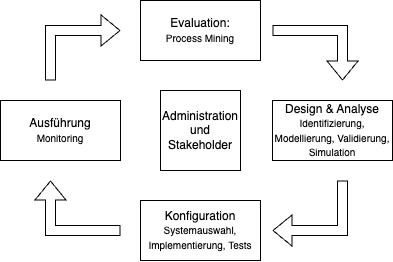
\includegraphics[width=\textwidth]{../assets/images/BPM-Lebenszyklus.drawio.png}
            \caption{BPM-Lebenszyklus nach \citet{Weske2019}.}
            \end{figure}
    
        Der Einstieg in den Zyklus ist die \textbf{Entwurfs- und Analysephase}, in der die Geschäftsprozesse identifiziert und in eine \gls{bpm} Repräsentation übersetzt wird. Die neu erstellten Modelle werden verifiziert und gegen aktuelle Prozessanforderungen validiert. In der \textbf{Konfigurationsphase} werden die zu verwendenden Systeme ausgewählt und die zuvor identifizierten Geschäftsprozesse implementiert, getestet und in Betrieb genommen. In der \textbf{Umsetzungsphase} werden die Prozesse betrieben, und die Prozessausführung wird überwacht und gepflegt. Die entstehenden Log-Dateien werden wiederum in der \textbf{Evaluationsphase} durch Processmining ausgewertet. Auf Grundlage der Ergebnisse wird eine neue Iteration begonnen.
    
    \section{Robotic Process Automation} \label{rpa}
    \gls{rpa} beschreibt Softwareroboter, welche auf der Benutzeroberfläche auf der gleichen Weise wie ein Mensch operiereren. \citet{vanderAalst2018} beschreibt \gls{rpa} als \say{[...] ein Oberbegriff für Werkzeuge, die auf der Benutzeroberfläche anderer Computersysteme in der Art und Weise bedienen, wie es ein Mensch tun würde}. Dabei können die Softwareroboter ohne umfangreiche Programmierkenntnisse als low-code Lösung implementiert werden, sodass diese schnell von Fachabteilungen ohne tiefergreifenden IT-Kenntnisse umgesetzt werden können, um Legacy-Systeme zu automatisieren. Im Gegensatz zu traditioneller Prozessautomatisierung kann \gls{rpa} Prozesse automatisieren, die keine API anbieten. Außerdem bietet es den Vorteil gegenüber manuellen Prozessen kostengünstiger, schneller und fehlerfreier Prozesse durchzuführen, sodass sich ein gesteigerter Return-On-Investment (ROI) ergibt \citep{Kroll2017}. Es haben sich jedoch auch eine Reihe von Problemen mit \gls{rpa} gezeigt: Um RPA-Prozess zu identifizieren und zu implementieren, ist umfangreiches Prozesswissen erforderlich. Ist dieses Wissen nicht vorhanden - da es beispielsweise an Systemen zum Erfassen dieses Wissens mangelt - werden die Vorteile von \gls{rpa} enorm geschmälert \citep[S.4f]{König2020RPA-BPMS}. Zudem können die eingesetzten Softwareroboter sehr fragil sein, da sie auf der Benutzeroberfläche operieren. Sobald sich Benutzeroberflächen ändern, scheitern diese. Dies schließt \gls{rpa} generell für kritische Geschäftsprozesse aus. Bei großflächig eingesetzten Softwarerobotern bedeutet das eine zeitintensive und kostspielige Wartungsarbeit \citep{Ruha2023}. Aufgrund des verstreuten Prozesswissens mangelt es oft auch an Information, welche Prozesse überhaupt geeignet sind, automatisiert zu werden \citep{Greene2019}. Der Scope von \gls{rpa} ist generell wesentlich enger zu fassen; es werden viel eher einzelne Prozessschritte eines komplexen Geschäftsprozess automatisiert, als die End-to-End Prozesse selbst \citep{Signavio2019}. \citet[S. 3]{König2020RPA-BPMS} schreibt hierzu: \say{Da RPA-Systeme nur Prozesse auf einer niedrigen 
    Abstraktionsebene automatisieren können, können RPA-Prozesse als Aktivitäten eines übergeordneten Geschäftsprozesses betrachtet werden.}

    \section{BPMS-RPA}
    Um die in \ref{rpa} beschriebenen Probleme zu lösen, gibt es aus der Forschung Vorschläge, Funktionalitäten von \gls{rpa} tiefer mit \gls{bpms} zu integrieren \citep{Flechsig2019}. Ein ähnliches Konzept lässt sich bei citet{Kirchmer2019} mit ihrem \say{value-driven robotic process automation} Ansatz finden, der einen ganzheitlichen Blick auf unternehmensweite Automatisierung wirft. Auch Gartner sieht im Konzept der Hyperautomation - eine Erweiterung von \gls{rpa} durch KI- und Integrationslösungen - den Bedarf an BPM-Lösungen, um Prozesse effinzienter und End-to-End automatisieren zu können \citep{Gartner2024}. Mögliche Vorteile einer BPMS-RPA Integration könnten einheitliches Prozesswissen, verbesserte Prozessoptimierung, robustere Fehlerbehandlung und Skalierbarkeit von Prozessautomatisierungen darstellen \citep[S. 2]{Flechsig2022Umfrage}. Auch wenn noch nicht weit verbreitet unter RPA-Lösungen, kann \gls{bpm} als Standardnotation das Bindeglied zwischen dem Management von Geschäftsprozessen und der Automatisierung selbiger darstellen \citep{Völker2021}. Unternehmen haben erkannt, dass die zunehmende Anzahl an Softwarerobotern eine standardisierte Orchestration bedarf, um die Ausführung von Geschäftsprozessen und RPA-Abläufen aufeinander abzustimmen. Dennoch werden in der Praxis  getrennte Systeme für \gls{rpa} und \gls{bpm} eingesetzt und auch organisatorisch sind die Themen innerhalb des Unternehmens getrennt \citep[S. 6ff]{Flechsig2022Umfrage}. Um eine tiefergreifende BPMS-RPA Integration im Unternehmen zu etablieren, stellt \citet{Flechsig2022Umfrage} eine Reihe von Anforderungen auf: Essenziell für eine Integration ist ein gewisse BPM-Reife (\say{BPM-Maturity}) des Unternehmens. Erst wenn Funktionen wie Prozessmodellierung, -einführung, -optimierung und -management erfolgreich im Unternehmen und der Unternehemenskultur etabliert wurden, lässt sich über eine tiegergehende BPMS-RPA Integration nachdenken. Darüberhinaus wird das generelle Mindset und die Offenheit dem Thema gegenüber betont. Oft sehen Unternehmen ein entweder-oder zwischen \gls{bpm} und \gls{rpa}


    Existing research suggests to solve these problems by combining RPA withbusiness process management (BPM). More specific, most works propose inte-grating RPA with BPM. RPA is considered more successful, or even only suc-cessful, when combined with BPM
    Gartner sieht im Konzept der Hyperautomation - eine durch generative KI erweiterte, hochskalierbare RPA-Lösung zur vollständigen End-to-End Automatisierung von Geschäftsprozesse - eine mögliche Verbesserung von bestehenden RPA-Lösungen, konkrete Ergebnisse und Evaluationen stehen jedoch noch aus 
- Vorschlag, beide Technologien zu verbinden
- beide Technolgien haben Gemeinsamkeiten, beide bauen auf Prozesse auf, haben die gleichen Ziele
- sind im Moment jedoch völlig getrennt: Though these technologies are very often used separately, the authors from business practice [14, 36] strongly suggest combining both to gain even more business value. In a case of the lack of resources and/or time to completely implement BPMS, RPA can
4 be a valuable and relatively inexpensive tool to solve or complement some of the un-fulfilled goals.
- BPM kann Rahmen schaffen, damit RPA schneller skalieren kann
- BPMN Notation könnte Brücke bilden
- somit ist: As RPA systems can only automate processes on a low level
of abstraction, RPA processes can be considered activities of a parent business
process.
- kann Probleme von RPA lösen
BPMNS-RPA kann eine Möglichkeit sein.
\subsection{BPMN-RPA Lifecycle}
- der in Kapitel 1 beschriebene Prozess lässt sich erweitern

\chapter{Marktübersicht}
-CAGR von BPM und RPA
- Marktgröße angeben
- Vendoren vorstellen
- dokumente einfließen lassen
- Fazit: noch keine tiefergreifende Integrationen
\begin{comment}
BPM market analysis
The BPM market was valued at $16 billion in 2023. Additionally, the market is projected to exceed $58 billion by the end of 2036, exhibiting 11 percent CAGR during the forecasted period. Some of the growth propelling factors for the market are:

A surge in focus on digitization of business processes.
The rapid adoption of BPM solutions for streamlining operations.
Increase in the adoption of cloud solutions.
The quest to raise the productivity of the business.
Furthermore, the market in the North America region is projected to reach almost 32 percent by the year 2036. The growth of the market can be attributed to the high penetration of advanced technologies among businesses. The presence of market leaders in the region is contributing to the significant development of various process modeling platforms. 
\end{comment}
- Reihe von Anbietern auf RPA und BPMN Seite,
- es wird untersucht, in wie fern die Anbieter Methoden beider Disziplinen vereinen.
- untersucht werden folgende:
\chapter{Fallstudie: BPMN Datenaustausch zwischen SAP Build Process Automation und SAP Signavio}
    - es wird ein Feature vorgestellt, das aktiv evaluiert wird.
    - reiht sich in den Bereich RPA-BPM ein (Interview angeben)
    - RPA-BPM wird von SAP als strategisch wichtig angesehen
    - 
    - Überleitung zum Hauptteil der Studienarbeit
    - Thema: BPMN dateien durch native Integration von SAP Signavio zu SAP Build Process Automation transferieren
    -SAP Signavio ist die BPMNS Lösung von SAP (daten: )
    - SAP Build Process Automation ist die RPA Lösung von SAP (daten?)
    - 
\section{SAP Signavio}
\section{SAP Build Process Automation}

\section{Problem Statement}
    - Kunden haben gleiche Probleme wie in Kapitel 1 angesprochen
        - Prozesse und Prozessinformationen sind voneinander getrennt (hier Insights einfügen (3 Stück))
    - auch organisatorisch sind COE RPA und COE BPMN getrennt voneinander
    - jetziges Szenario: Prozess-Team entdeckt manuellen Prozess in Signavio Process Insights, dann muss es Automatisierungs-team kontaktieren, dann muss das Team den Prozess bekommen und nochmal modellieren
    - das ist nicht gut, zu langsam, fehlende Kommunikation
    - Kunde wünscht sich eine bessere Integration, mehr Automatisierung

    - hier auf die angeführten Probleme aus Kapitel 1 eingehen
    - Personas vorstellen
    - User Demand angeben


   \section{Integration}
   - die stärkere kollaboration zwischen Signavio Process Manager und SBPA kann als Schritt in Richtung BPMS-RPA verstanden werden
   - damit besteht die Mögllichkeit für SAP, auf dem Gebiet vorreiter zu werden
   - Sie kann die in Kapitel 1 beschriebenen Probleme lösen
   - einen einheitlichen ende-zu-ende Prozess darstellen und rpa skalierbar machen
   - ein erster Versuch ist folgendes Feature:
   - es wird überprüft, in wie fern ein automatischer BPMN Datenaustausch zwischen Signavio und SBPA zu realisieren ist.
   - als MVP wird der manuelle BPMN import gesetzt
   - Nach Evaluation des MVPs sind weitere tiefergreifende Integrationen vorstellbar

   - hier auf den POC eingehen
    .Es wird eine Integration evaluiert, um signavio und sbpa stärker zu integrieren
\subsection{Technische Voraussetzung}
- sbpa hat eine workflow engine, die bpmn2.0 compliant ist, basiert auf xxx engine
- jedoch werden in der design time der Anwendung nicht alle shapes unterstützt.
-hier tabelle mit shapes einfügen

   - welche optionen werden evaluiert?
    - eine iflow Integration
    - einen bpmn Import
    - eine native Integration
    - auf den lifecycle eingehen
    - ea story erzählen
    
    \section{To-Be Modellierung}
    - User Journey?
    - man identifiziert einen manuellen Prozess in Signavio
    - Der Prozess zeigt ein hohes Automatisierungspotential an
    - man kann den Prozess zunächst manuell herunterladen
    - dann bei SBPA importieren
    - in SBPA anpassen, RPA-Bots, Connectoren, usw. einbinden
    - Prozess testen
    - man hat einen manuellen Prozess automatisiert, ohne ihn doppelt zu modellieren
    - UI Mockups einbinden
    \section[short]{SAP Enterprise Automation}
    - EA als RPA-BPMNS bestreben von SAP
\chapter{Ausblick}
    \section{Bewertung}
    - manueller Import immer noch zu aufwendig
    - nicht alle Artefakte lassen sich übertragen
        - man muss trotzdem viel in SBPA anpassen
        - darum ist keine Synchronisation möglich
    \section{Weiterentwicklung}
    \section{Weitere Integrationsszenarien}

%Schluss
{\let\clearpage\relax \chapter{Fazit}} 




\newpage
\pagenumbering{Roman}
\setcounter{page}{\number\value{originalpagenumber}}


%Literaturverzeichnis

\nocite{*}

%Anhang
\newpage
\printbibliography

hallo


%Ehrenwörtlich erklährung 
\chapter*{Ehrenwörtliche Erklärung}
\addcontentsline{toc}{chapter}{Ehrenwörtliche Erklärung}

% Keine Kopf- und Fußzeilen ausgeben
\thispagestyle{empty}
% Aber trotzdem ins Inhaltsverzeichnis aufnehmen
%\addcontentsline{toc}{section}{Eidesstattliche Erklärung}

% Hier der offizielle Text der eidesstattlichen Erklärung
Ich erkläre ehrenwörtlich:
\begin{enumerate}
	\item dass ich die Hausarbeit selbstständig verfasst habe,
	\item dass ich die Übernahme wörtlicher Zitate aus der Literatur sowie die Verwendung der Gedanken anderer Autoren an den entsprechenden Stellen innerhalb der Arbeit gekennzeichnet habe,
	\item dass ich den Hausarbeit bei keiner anderen Prüfung vorgelegt habe.
\end{enumerate}
Ich bin mir bewusst, dass eine falsche Erklärung rechtliche Folgen haben wird.
% Etwas Abstand für die Unterschrift
\vspace{2cm}

% Hier kommt die Unterschrift drüber
\begin{tabular}{lp{4em}l} 
 \hspace{5cm}   && \hspace{4cm} \\\cline{1-1}\cline{3-3} 
 Ort, Datum     && \studentName
\end{tabular}


\end{document}
